\documentclass[10pt]{report}
\usepackage[a4paper, left=2cm, right=2cm]{geometry}
\usepackage{xcolor}
\definecolor{grey}{rgb}{0.9,0.9,0.9}
\usepackage[utf8]{inputenc}
\usepackage[T1]{fontenc}
\usepackage[sfdefault,light]{FiraSans}
\usepackage{graphicx}
\usepackage{colortbl}

\usepackage{enumerate}

\usepackage{titlesec}
\titleformat{\chapter}[display]   
{\normalfont\huge\bfseries}{\chaptertitlename\ \thechapter}{20pt}{\Huge}   
\titlespacing*{\chapter}{0pt}{-50pt}{40pt}

\renewcommand{\theenumii}{\theenumi.\arabic{enumii}}
\renewcommand{\labelenumi}{\theenumi.}
\renewcommand{\labelenumii}{\theenumii.}
\renewcommand{\contentsname}{Spis treści}
\usepackage{hyperref}
\hypersetup{
	colorlinks,
	citecolor=black,
	filecolor=black,
	linkcolor=black,
	urlcolor=black
}
\renewcommand{\chaptername}{}
\addtocontents{toc}{\protect\setcounter{tocdepth}{1}}
\begin{document}
	
	\begin{titlepage} 
		
		\begin{center}
			
\includegraphics[scale=0.4]{agh.jpg}
		\end{center}

		\vfill
			\colorbox{grey}{
				\parbox[t]{0.93\textwidth}{
					\parbox[t]{0.91\textwidth}{
						\raggedleft
						\fontsize{50pt}{80pt}\selectfont
						\vspace{0.7cm}
						Coffeeland\\
						\fontsize{20pt}{50pt}\selectfont
						Projekt sklepu internetowego\\
						\fontsize{15pt}{30pt}\selectfont
						Inżynieria Oprogramowania\\
						\vspace{0.7cm}
				}
			}
		}
	
		\vfill
		\parbox[t]{0.93\textwidth}{
			\raggedleft
			\large
			{\Large Aneta Pociecha}\\[4pt]
			{\Large Magdalena Tragarz}\\[4pt]
			{\Large Marek Ochocki}\\[4pt]
			{\Large Artur Bugaj}\\[4pt]
		}
		
	\end{titlepage}
	
	
	\tableofcontents
	
	\setcounter{chapter}{0}	
	\setcounter{section}{0}	

	\chapter{Ogólny opis systemu}
	

		\section{Cel systemu}
	
		Celem realizowanego systemu jest stworzenie prostego w użyciu sklepu internetowego z kawą. Zakupy wymagają założenia konta. Wybór produktów odbywa się poprzez katalog znajdujący się na stronie głównej. Klikając na produkt można przejść do osobnej strony ze szczegółowymi informacjami. Dodawanie produktów do koszyka odbywa się z poziomu podstrony produktu. W koszyku klient ma możliwość złożenia zamówienia. Płatność jest realizowana poprzez system PayPal. W sklepie został przewidziany system reklamacji.
		
		\section{Lista możliwości}
		\begin{itemize}
			\item rejstracja użytkownika
			\item logowanie użytkownika
			\item zakup produktu
			\item reklamacja
			\item filtrowanie oferty ze względu na typ produktu i zakres ceny
			\item zapis do newslettera
			\item rezygnacja z newslettera
			\item dodanie adresu do listy adresów
			\item usunięcie adresu z listy adresów
			\item edycja danych użytkownika
		\end{itemize}
	

		\section{Diagram kontekstowy}
			\begin{center}
				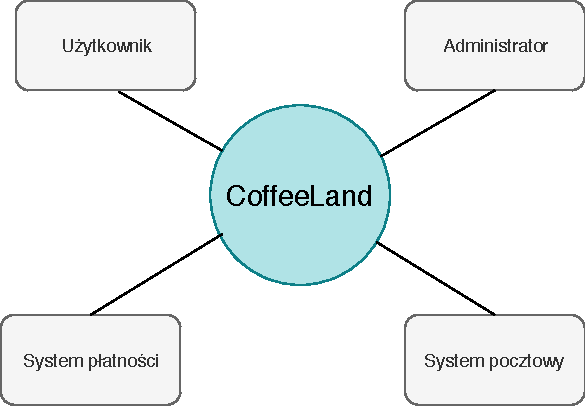
\includegraphics[width=280pt]{kontekstowy.pdf}
			\end{center}
	

		\section{Warstwy systemy}
			\begin{center}
				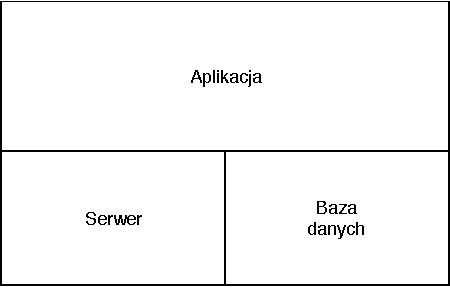
\includegraphics[width=250pt]{layers.pdf}
			\end{center}
		

	\renewcommand{\thesection}{\thechapter.\arabic{section}}	
	

	
\chapter{Analiza i projekt}


\section{Interfejsy}


\subsection{Interfejs serwera}

\subsubsection{Commands}

\begin{enumerate}
	\item RegisterNewClientCommand
	\item UpdatePersonalDataCommand
	\item AddAddressCommand
	\item InactivateAddressCommand
	
\end{enumerate} 

	
\subsubsection{Queries}
\begin{enumerate}
	\item GetPersonalDataQuery
	\item GetShopItemsQuery
	\item GetAddressBookQuery
	\item GetOrdersQuery
	\item SignInQuery
	\item SignOutInQuery
\end{enumerate}	



\subsection{Interfejs użytkownika}

\begin{enumerate}
	\item Filtr
	\item Dodanie produktu do koszyka
	\item Wybór ilości danego produktu
	\item Formularz rejestracji
	\item Formularz logowania
	\item Formularz edycji danych osobowych
	\item Formularz dodania adresu
	\item Zapis/wypis do/z newsletter'a
	\item Usunięcie adresu
	\item Usunięcie towaru z koszyka
	\item Formularz reklamacji
	\item Formularz zakupu
	
\end{enumerate} 

\subsection{Testy automatyczne}
Testom automatycznym zostały poddane następujace funkcjonalności:
\begin{enumerate}
	\item Filtr
	\item Dodanie produktu do koszyka
	\item Wybór ilości danego produktu
	\item Formularz rejestracji
	\item Formularz edycji danych osobowych
	\item Formularz dodania adresu
	\item Zapis/wypis do/z newsletter'a
	\item Usunięcie adresu
	\item Usunięcie towaru z koszyka
	\item Formularz reklamacji
	
\end{enumerate} 

	
	\section{Diagram komponentów}
	\begin{center}
		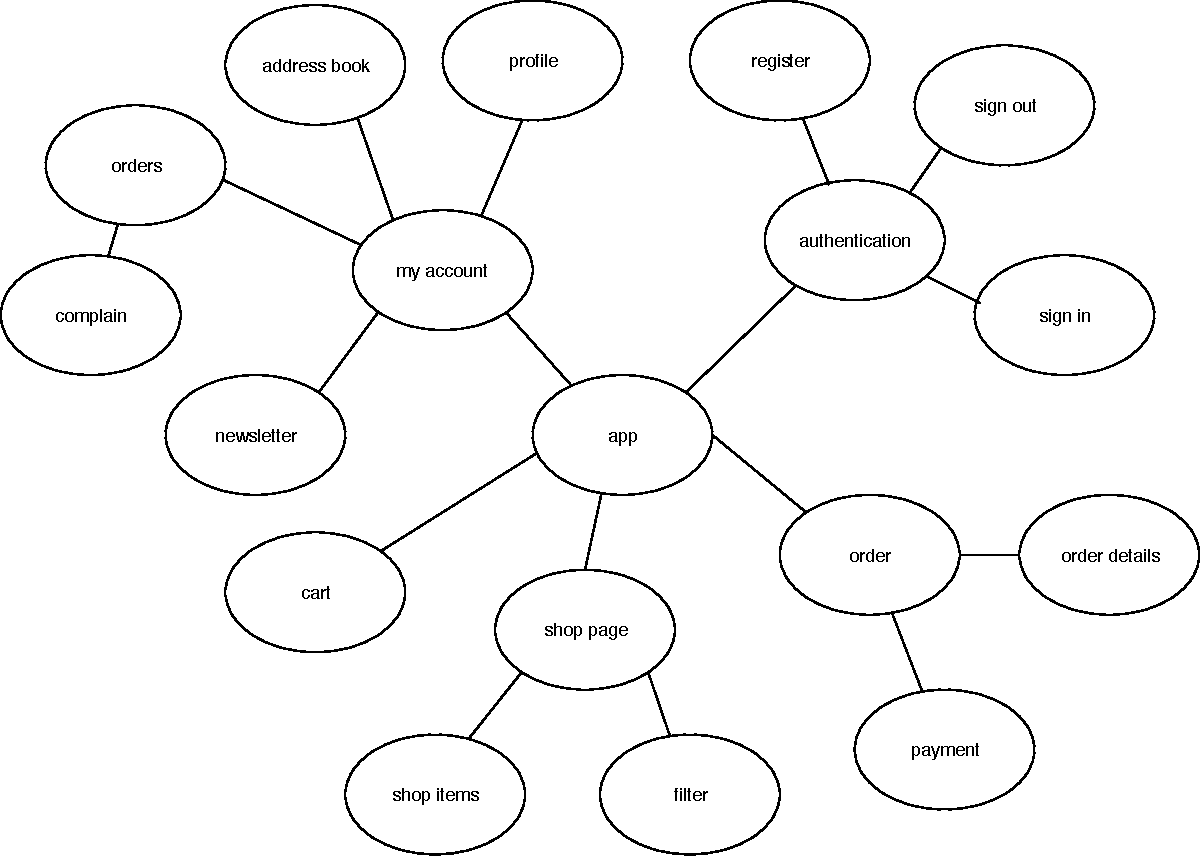
\includegraphics[width=500pt]{components.pdf}
	\end{center}


	\section{Projekt bazy danych}
		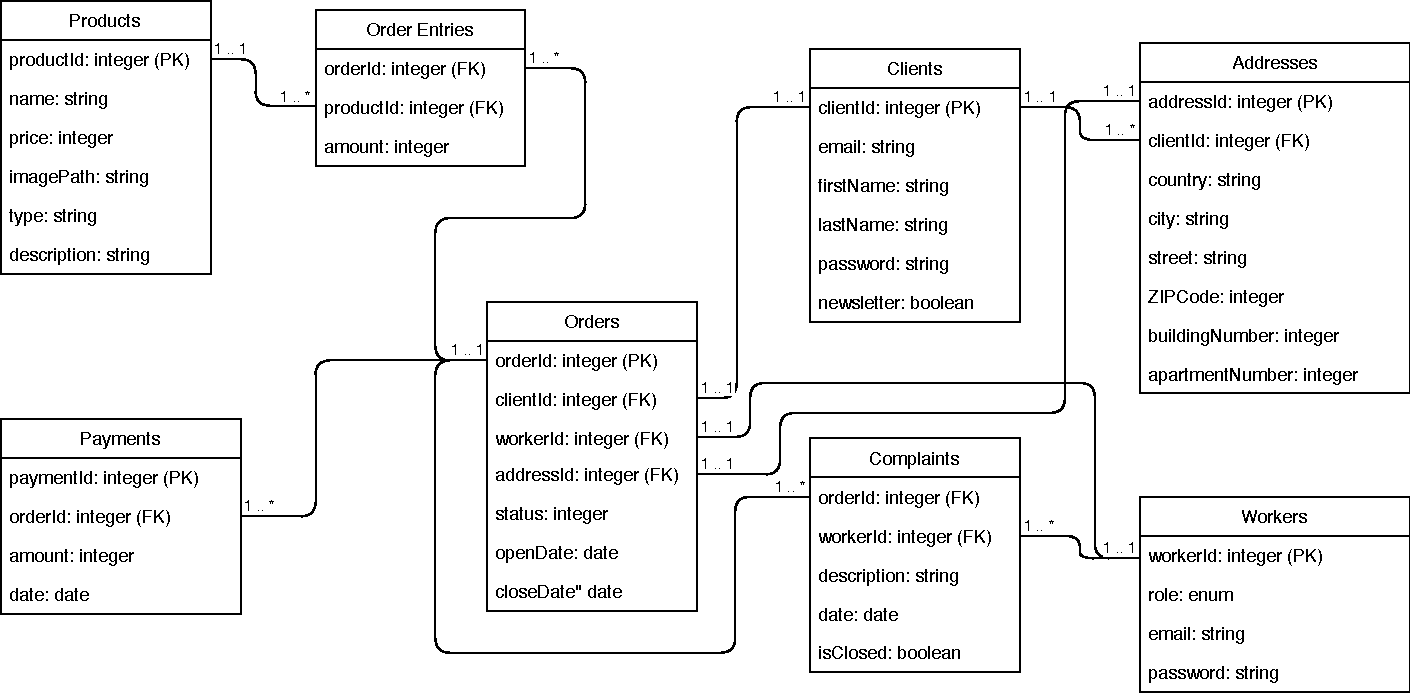
\includegraphics[width=500pt]{database.pdf}
		 


\section{Słownik danych}

		\paragraph{country} $=$ 2-30 liter
		\paragraph{city} $=$  2-30 liter
		\paragraph{street} $=$ 0-30 liter
		\paragraph{ZIPCode} $=$ <cyfra><cyfra>-<cyfra><cyfra><cyfra>
		\paragraph{Building number} $=$ 1-6 cyfry
		\paragraph{Apartament number} $=$ 0-10 cyfr lub liter
		\paragraph{Letter of complain} $=$  minimum 10 znaków
		\paragraph{email} $=$ <minimum jeden znak> @ <minimum jeden znak> .  <minimum jeden znak>
		\paragraph{hasło} $=$ minimum 8 znaków w tym wielka litera, mała litera i cyfra 
		\paragraph{imię}  $=$ od 2 do 10 liter
		\paragraph{nazwisko} $=$ od 2 do 10 liter

	
\section{Technologie i narzędzia}

\begin{itemize}
	\item ReactJS
	\item JavaScript
	\item SignalR 
	\item nUnit  
	\item .NET 
	\item Jest
	\item git
	\item Redux
	\item Visual Studio Code  
	\item Visual Studio Community 
	\item Chromium
	\item Selenium
	\item CircleCI
	\item GitHub 
	\item  Trello
	\item SQL
\end{itemize}

	
	
\end{document}